\documentclass[handout]{beamer}
% \documentclass{beamer}

%%
%%
%%
% From http://tex.stackexchange.com/questions/2072/beamer-navigation-circles-without-subsections
% Solution #2 or 3:
% \usepackage{etoolbox}
% \makeatletter
% % replace the subsection number test with a test that always returns true
% \patchcmd{\slideentry}{\ifnum#2>0}{\ifnum2>0}{}{\@error{unable to patch}}%
% \makeatother
% Solution #1:
\usepackage{remreset}% tiny package containing just the \@removefromreset command
\makeatletter
\@removefromreset{subsection}{section}
\makeatother
\setcounter{subsection}{1}


\usepackage{etex}
\usepackage{pgf}
\usepackage{tikz}
\usepackage{url}
\usepackage{amsmath}
\usepackage{color}
% \definecolor{red}{rgb}{1,0,0}
\usepackage{ulem}
% \usepackage{booktabs}
\usepackage{colortbl,booktabs}
\renewcommand*{\thefootnote}{\fnsymbol{footnote}}
\usepackage{fancybox}
\usepackage[framemethod=TikZ]{mdframed}
\mdfdefinestyle{FactStyle}{%
  outerlinewidth=0.5,
  roundcorner=1pt,
  leftmargin=1cm,
  linecolor=blue,
  outerlinecolor=blue!70!black,
  backgroundcolor=yellow!40
}
\usepackage{cancel}

  \newcommand\Warning{%
    \makebox[2.4em][c]{%
      \makebox[0pt][c]{\raisebox{.2em}{\Large!}}%
      \makebox[0pt][c]{\color{red}\Huge$\bigtriangleup$}}}%

\usepackage{stackengine}
\usepackage{scalerel}
\usepackage{xcolor}
  \newcommand\dangersign[1][2ex]{%
    \renewcommand\stacktype{L}%
    \scaleto{\stackon[1.3pt]{\color{red}$\triangle$}{\tiny !}}{#1}%
  }



\usepackage{dcolumn}
\newcolumntype{d}[1]{D{.}{.}{#1}}

% From
% http://tex.stackexchange.com/questions/109900/how-can-i-box-multiple-aligned-equations
\usepackage{empheq}
\usepackage{tcolorbox}  \newtcbox{\othermathbox}[1][]{%
  nobeforeafter, tcbox raise base, 
  colback=black!10, colframe=red!30, 
  left=1em, top=0.5em, right=1em, bottom=0.5em}

\newcommand\blue{\color{blue}}
\newcommand\red{\color{red}}
\newcommand\green{\color{green!75!black}}
\newcommand\purple{\color{purple}}
\newcommand\bluegreen{\color{blue!75!green}}
\newcommand\orange{\color{orange}}
\newcommand\redgreen{\color{red!50!green}}
\newcommand\grey{\color{black}}
\newcommand\gap{\vspace{.1in}}
\newcommand\nb{${\red\bullet}\ $}
\newcommand\halfgap{\vspace{.05in}}
\newcommand\divideline{\line(1,0){352}}
\usepackage{marvosym} % for \Smiley

\newcommand{\bluealert}[1]{{\blue\textbf{#1}}}

% \usepackage{beamerthemesplit} %Key package for beamer
\usetheme{Singapore}
% \usetheme{Szeged}
% \usetheme{Garfield}
% \usetheme{CambridgeUS}
% \usenavigationsymbolstemplate{} %Gets rid of slide navigation symbols


\setbeamercolor{separation line}{use=structure,bg=structure.fg!50!bg}
% \begin{beamercolorbox}[colsep=0.5pt]
%   {upper separation line foot}
% \end{beamercolorbox}



\makeatletter
\setbeamertemplate{footline}
{
  \leavevmode%
  \hbox{%
% \begin{beamercolorbox}[colsep=0.5pt]
%   {upper separation line foot}
% \end{beamercolorbox}


  \begin{beamercolorbox}[wd=.5\paperwidth,ht=2.25ex,dp=2ex,colsep=0.5pt]%
    {upper separation line foot}
    \usebeamerfont{author in head/foot}%
    \hspace*{2ex}\insertshortdate:\ \insertshorttitle
  \end{beamercolorbox}%
  \begin{beamercolorbox}[wd=.5\paperwidth,ht=2.25ex,dp=2ex,right]{title in head/foot}%
    \usebeamerfont{title in head/foot}
    {\insertshortauthor}\hspace*{2ex}
  \end{beamercolorbox}}%
  % \begin{beamercolorbox}[wd=.333333\paperwidth,ht=2.25ex,dp=2ex,right]{date in head/foot}%
  %   \usebeamerfont{date in head/foot}\insertshortdate{}\hspace*{2em}
  %   \insertframenumber{} / \inserttotalframenumber\hspace*{2ex} 
  % \end{beamercolorbox}%
  \vskip0pt%
}
\makeatother

\usetikzlibrary{decorations.markings}
\usetikzlibrary{arrows}


\title{Final Exam Review}
\author{Peter Garfield, UCSB Mathematics}
\date{March 15, 2017}
%\institute{}


\useinnertheme{default}

\usefonttheme{serif}
% \usecolortheme{rose}
% \usecolortheme{whale}
% \usecolortheme{orchid}
\usecolortheme{crane}
% \usecolortheme{dolphin}


%TEMPLATE
\setbeamertemplate{navigation symbols}{}

\setbeamertemplate{note page}[compress]

\setbeamertemplate{frametitle}{
  \vspace{0.5em}
  % \begin{centering}
  {\huge\blue\textbf{\textmd{\insertframetitle}}}
  \par
  % \end{centering}
}

% From http://tex.stackexchange.com/questions/7032/good-way-to-make-textcircled-numbers:
\newcommand*\circled[1]{\tikz[baseline=(char.base)]{\node[shape=circle,draw,fill=orange,inner sep=1pt] (char) {#1};}} 
% \renewcommand{\labelenumi}{\circled{\textbf{\arabic{enumi}}}}

\let\olddescription\description
\let\oldenddescription\enddescription
\usepackage{enumitem}
\let\description\olddescription
\let\enddescription\oldenddescription

% \usepackage[loadonly]{enumitem}
\setlist[enumerate,1]{label=\colorbox{orange}{\arabic*.},font=\bfseries}
%\setlist[enumerate,2]{label=\colorbox{blue!25}{(\alph*)},font=\bfseries}
% \setlist[enumerate,1]{label=\arabic*.,font=\bfseries}
\setlist[itemize,1]{label=\red$\bullet$}
\setlist[itemize,2]{label=\blue$\bullet$}

\newcommand\answer[1]{\fbox{#1}}
% \renewcommand\answer[1]{}

\newcommand{\antilog}{\operatorname{antilog}}







\title{}
\title{Understanding Derivatives}
\date{May 15, 2017}


\begin{document}
\small

\section*{Administration}

\frame{
  \frametitle{Office Hours!}
  % \ \vspace*{0.25in}

  {\Large{}Instructor:}\\
  \ \hspace*{0.2in} Peter M.\ Garfield, \url{garfield@math.ucsb.edu}\\[0.25em]

  {\Large{}Office Hours:}\\
  \ \hspace*{0.2in} Mondays 2--3\textsc{pm}\\
  \ \hspace*{0.2in} Tuesdays 10:30--11:30\textsc{am}\\
  \ \hspace*{0.2in} Thursdays 1--2\textsc{pm}\\
  \ \hspace*{0.2in} or by appointment \\[0.25em]

  {\Large{}Office:}\\
  \ \hspace*{0.2in} South Hall 6510\\[0.5em]

  \copyright\ 2017\ Daryl Cooper, Peter M.\ Garfield

  % \vspace*{2in}
}

\section{Review}

\frame{
  \frametitle{Graphical Approach}

  \begin{minipage}{0.5\linewidth}
    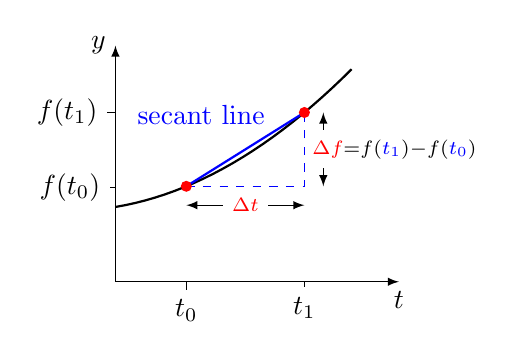
\begin{tikzpicture}[x=12mm,y=12mm,>=latex]
        \draw[black,->] (0,0) -- (3,0) node[below] {$t$};
        \draw[black,->] (0,0) -- (0,2.5) node[left] {$y$};
        % Ticks:
        \draw[thin,black] (0.75,0) -- (0.75,-3pt) node[below] {$t_0$};
        \draw[thin,black] (2,0) -- (2,-2pt) node[below] {$t_1$};
        \draw[thin,black] (0,1) -- (-2pt,1) node[left] {$f(t_0)$};
        \draw[thin,black] (0,{0.75+(2+1/2)^2/6}) -- (-3pt,{0.75+(2+1/2)^2/6}) node[left] {$f(t_1)$};
        \draw[black,thick] plot[domain=0:2.5] (\x,{0.75+(\x+1/2)^2/6});
      %
        \draw[thick,blue] (0.75,{0.75+(0.75+1/2)^2/6}) -- (2,{0.75+(2+1/2)^2/6}) node[near end,left,yshift=2mm] {secant line};
        \draw[thin,black,<->] (0.75,{0.75+(0.75+1/2)^2/6-0.2}) -- (2,{0.75+(0.75+1/2)^2/6-0.2}) node[midway,red,fill=white] {$\scriptstyle\Delta t$};
        \draw[thin,black,<->] (2.2,{0.75+(0.75+1/2)^2/6}) -- (2.2,{0.75+(2+1/2)^2/6}) node[midway,fill=white,right,xshift=-0.75em] {$\scriptstyle{\red\Delta f}=f({\blue t_1})-f({\blue t_0})$};
        \draw[thin,blue,dashed] (0.75,{0.75+(0.75+1/2)^2/6}) -- (2,{0.75+(0.75+1/2)^2/6}) -- (2,{0.75+(2+1/2)^2/6});
        % 
      %
        \fill[red] (0.75,{0.75+(0.75+1/2)^2/6}) circle (2pt);
        \fill[red] (2,{0.75+(2+1/2)^2/6}) circle (2pt);
    \end{tikzpicture}
  \end{minipage}
  \hfill
  \parbox{50mm}{%
    ${\red\Delta f}=$ change in $f$ \\
    ${\red\Delta t}=$ change in $t$\\[0.5em]
    \alert{Many ways to say same thing:}\\
    $\begin{array}{l}
       \left(\begin{array}{c} \text{{\blue average} rate of}\\ \text{change of $f$}\end{array}\right)  = \dfrac{\text{change in $f$}}{\text{change in $t$}}\\
       = \dfrac{\red \Delta f}{\red\Delta t}\\
       =  \text{slope of {\blue secant line}}
       = \dfrac{f({\blue t_1})-f({\blue t_0})}{{\blue t_1}-{\blue t_0}}
     \end{array}$
   }
   \pause

   The derivative is defined to be
   \begin{equation*}
     \lim_{\Delta t\to0} \left(\frac{\red\Delta f}{\red\Delta t}\right) 
     = \frac{df}{dt}
   \end{equation*}
   \pause

   Idea: As $t_1$ moves closer to $t_0$ the secant line approaches the {\blue tangent line}  at $t_0$.
   This is the line with the {\blue same slope} as the graph at $t_0$.

   % \fbox{{\red Let's watch a movie }} \qquad\qquad  No, not  {\blue The Bourne Identity}  :(\\

   % http://www.youtube.com/watch?v=AdQG2iSLDjA\\
   % http://www.youtube.com/watch?v=s3q8D79bjiE\&feature=related
}



\frame{
  \frametitle{Understanding Derivatives}

  There are many ways to {\blue think} about derivatives.  You {\blue
    need} to understand these to apply to problems. 
  \gap
  \gap 

  \begin{minipage}{0.35\linewidth}
    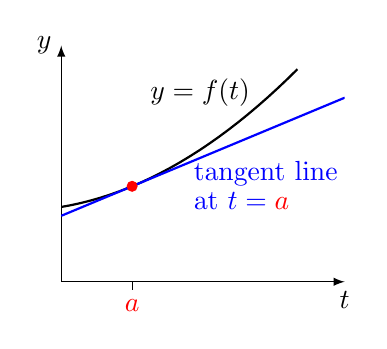
\begin{tikzpicture}[x=12mm,y=12mm,>=latex]
        \draw[black,->] (0,0) -- (3,0) node[below] {$t$};
        \draw[black,->] (0,0) -- (0,2.5) node[left] {$y$};
        % Ticks:
        \draw[thin,black] (0.75,0) -- (0.75,-3pt) node[below] {\red$a$};
        % \draw[thin,black] (2,0) -- (2,-2pt) node[below] {$t_1$};
        % \draw[thin,black] (0,1) -- (-2pt,1) node[left] {$f(t_0)$};
        % \draw[thin,black] (0,{0.75+(2+1/2)^2/6}) -- (-3pt,{0.75+(2+1/2)^2/6}) node[left] {$f(t_1)$};
        \draw[black,thick] plot[domain=0:2.5] (\x,{0.75+(\x+1/2)^2/6});
        \begin{scope}
          \clip (0,0) rectangle (3,2.5);
          \draw[blue,thick] plot[domain=0:3] (\x,{(0.75+1/2)*(\x-0.75)/3+0.75+(0.75+1/2)^2/6});
          \node[blue,right] at (1.3,1.15) {tangent line};
          \node[blue,right] at (1.3,0.85) {at $t={\red{}a}$};
          \node[left] at (2.1,2) {$y=f(t)$};
        \end{scope}
      %
      %
        \fill[red] (0.75,{0.75+(0.75+1/2)^2/6}) circle (2pt);
    \end{tikzpicture}
  \end{minipage}
  \hfill
  \parbox{60mm}{%
    slope of {\blue graph} at {\red a}\\
    = slope of {\blue tangent line} \\%\small{\red $\quad\quad^{discuss}$}\\
    = {\purple instantaneous rate of change} of $f$ at ${\red a}$\\
    \\
    $= \left(
      \begin{array}{l}
        \text{limit of average rate of change } \\ 
        \text{of $f$ over shorter and shorter}\\
        \text{ time intervals starting at\ {\red$a$}}
      \end{array}
    \right)$\\
    \\
    $=$ limit of slopes of secant lines\\
    $= f'({\red a})\ =\ \left. \dfrac{df}{dt}\right|_{t={\red a}}$
  }

}

\frame{
  \frametitle{Summary of Derivatives}

  One quantity, $\red y$, depends on another quantity $\blue x$. \\
  In other words $\red y$ is a {\blue function} of $\blue x$ so ${\red y}=f({\blue x})$.
  \hfill 
  \alert{Example:} ${\red y}={\orange 7}{\blue x}$
  \pause
  \gap

  If you change ${\blue x}$, then ${\red y}$ changes.

  \alert{Question:}\ How quickly does ${\red y}$ change as ${\blue x}$ changes? 
  \pause
  \gap

  Answer: The {\orange derivative} tells you. 
  \pause
  \gap 

  In our example, the derivative is $\orange 7$.  This tells you:
  \halfgap  

  \begin{center}
    {the {\red  output = $y$} of the function changes\\ 
      $\orange 7$ {\purple times} as fast\\ 
      as the {\blue input = $x$ } to the function.}
  \end{center}
  \gap
  \pause 

  If $\blue x$ is changed by $\blue 0.1$ how much does $\red y$ change by?
  \begin{center}
    A$=7$
    \quad 
    B$=7.1$
    \quad 
    C$=0.7$
    \quad 
    D$=0.1/7$
    \quad 
    E$=\text{other}$
    \quad
    \pause
    \fbox{C}
  \end{center}
}


\section{Meaning of Derivatives}

\frame{
  \frametitle{Graphical Meaning}

  \begin{minipage}{0.45\linewidth}
    \begin{empheq}[box=\othermathbox]{align*}
      \Large%
      \frac{d}{dx}\left( x^2\right) = 2x      
    \end{empheq}
    % \vspace{.1in}

    What this {\blue means}
    %% \vspace{.1in}

    \begin{empheq}[box=\othermathbox]{align*}
      \text{The {\red slope} of the graph\ }\\
      \text{of ${\blue y=x^2}$ at $x={\red a}$ is $2{\red a}$}
    \end{empheq}
  \end{minipage}
  \hspace*{0.25in}
  \begin{minipage}{0.45\linewidth}
    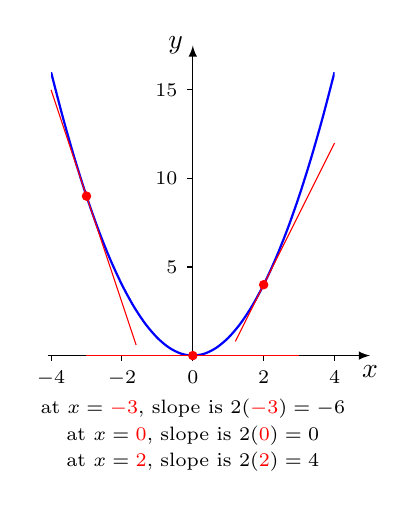
\begin{tikzpicture}[x=4.5mm,y=2.25mm,>=latex]
      \draw[thin,black,->] (-4.1,0) -- (5,0) node[below] {$x$};
      \draw[thin,black,->] (0,0) -- (0,17.5) node[left] {$y$};
      % ticks:
      \foreach \x in {-4,-2,0,2,4}
      {
        \draw[thin,black] (\x,0) -- (\x,-2pt) node[below] {$\scriptstyle\x$};
      }
      \foreach \y in {5,10,15}
      {
        \draw[thin,black] (0,\y) -- (-2pt,\y) node[left] {$\scriptstyle\y$};
      }
      \begin{scope}
        \clip (-4,0) rectangle (4,16);
        \draw[blue,thick,domain=-4:4,smooth] plot (\x,{(\x)^2});
      \end{scope}
      \uncover<2>{%
        \node at (0,-3) {$\scriptstyle\text{at $x={\red-3}$, slope is $2({\red-3})=-6$}$};
        % tangent line is y-9=-6(x+3) or y=-6x-9
        \draw[thin,red,domain=-4:-1.6] plot (\x,{-6*\x - 9});
        \filldraw[red] (-3,9) circle (1.5pt);
      };
      \uncover<3>{%
        \node at (0,-4.5) {$\scriptstyle\text{at $x={\red0}$, slope is $2({\red0})=0$}$};
        % tangent line is y=0
        \draw[thin,red] (-3,0) -- (3,0);
        \filldraw[red] (0,0) circle (1.5pt);
      };
      \uncover<4->{%
        \node at (0,-6) {$\scriptstyle\text{at $x={\red2}$, slope is $2({\red2})=4$}$};
        % tangent line is y-4=4(x-2) or y=4x-4
        \draw[thin,red,domain=1.2:4] plot (\x,{4*\x - 4});
        \filldraw[red] (2,4) circle (1.5pt);
      };
    \end{tikzpicture}
  \end{minipage}
  % \gap

  \uncover<5->{%
    \begin{empheq}[box=\othermathbox]{align*}
      \text{derivative}
      = \text{rate of change}
      = \text{slope of graph}
      = \text{slope of tangent line}
    \end{empheq}
  }



}

\frame{
  \frametitle{Slope Question}

  This graph shows $\red y=f(x)$ and lines parallel to $\blue y=2x$
  % \begin{center}
  %   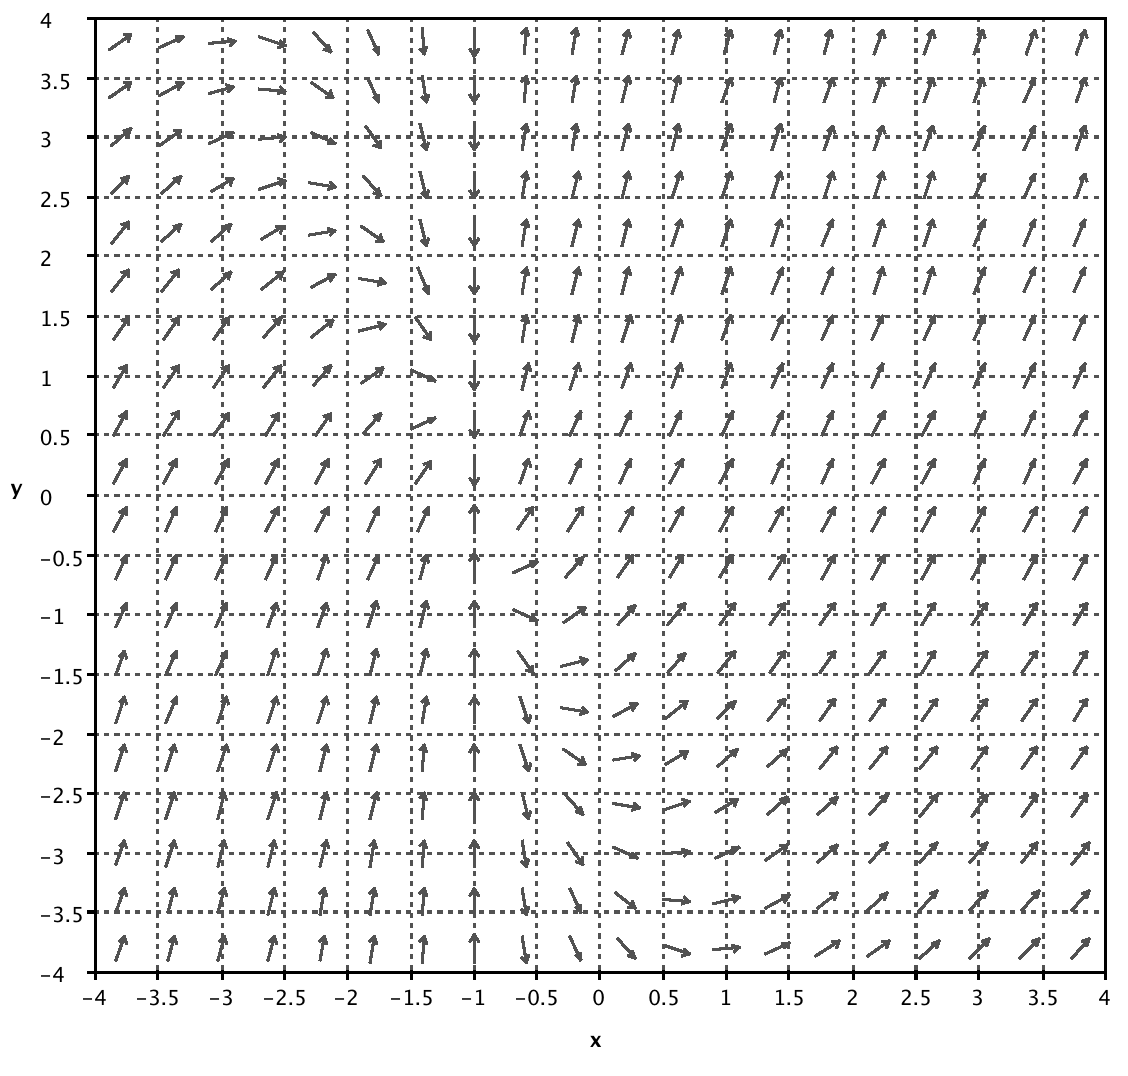
\includegraphics[scale=1]{slope.pdf}    
  % \end{center}
  \begin{center}
    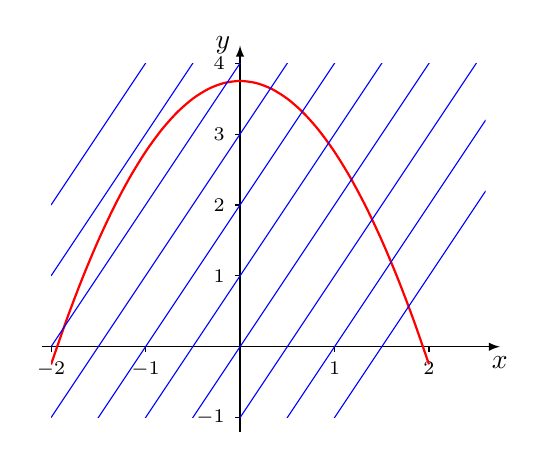
\begin{tikzpicture}[x=12mm,y=9mm,>=latex]
      \draw[thin,black,->] (-2.1,0) -- (2.75,0) node[below] {$x$};
      \draw[thin,black,->] (0,-1.2) -- (0,4.25) node[left] {$y$};
      %
      \foreach \x in {-2,-1,1,2}
      {
        \draw[thin,black] (\x,0) -- (\x,-2pt) node[below] {$\scriptstyle\x$};
      }
      \foreach \y in {-1,1,2,3,4}
      {
        \draw[thin,black] (0,\y) -- (-2pt,\y) node[left] {$\scriptstyle\y$};
      }
      \begin{scope}
        \clip (-2,-1) rectangle (2.6,4);
        \draw[thick,red,domain=-2:2,smooth] plot (\x,{3.75-(\x)^2});
        \foreach \k in {-3,-2,...,6}
        {
          \draw[thin,blue,domain=-2:2.6] plot (\x,{2*\x+\k});
        }
      \end{scope}
    \end{tikzpicture}
  \end{center}

  \alert{Question:}\ For which values of $x$ is ${\red f'(x)} > 2$?
  \begin{center}
    A\ $x<1.2$
    \quad 
    B\ $x<0$
    \quad 
    C\ $x<-1.5$
    \quad 
    D\  $x<-1$
    \quad 
    E\  $x < -0.5$
    \pause
    \quad
    \fbox{D}
  \end{center}

  % \gap Look for point on curve where curve parallel to blue line. That is the answer.


}

\frame{
  \frametitle{More Slope Questions}
  \begin{center}
    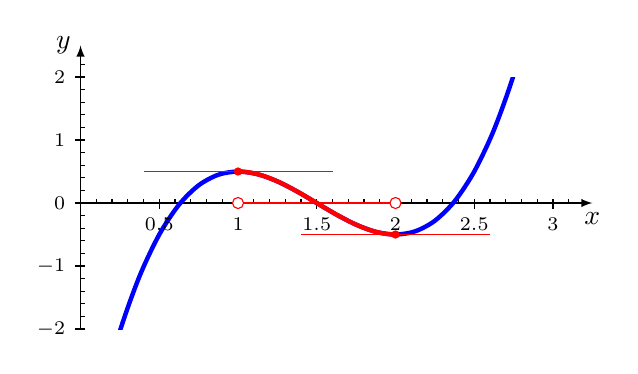
\begin{tikzpicture}[x=20mm,y=8mm,>=latex]
      \draw[thin,black,->] (0,0) -- (3.25,0) node[below] {$x$};
      \draw[thin,black,->] (0,-2) -- (0,2.5) node[left] {$y$};
      \begin{scope}
        \clip (0,-2) rectangle (3,2);
        \draw[ultra thick,blue,domain=0:3,smooth] plot (\x,{2*(\x)^3-9*(\x)^2+12*\x-4.5});
      \end{scope}
      \foreach \x in {0.5,1,1.5,2,2.5,3}
      {
        \draw[thin,black] (\x,0) -- (\x,-2pt) node[below] {$\scriptstyle\x$};
      }
      \foreach \y in {-2,-1,0,1,2}
      {
        \draw[thin,black] (0,\y) -- (-2pt,\y) node[left] {$\scriptstyle\y$};
      }
      \foreach \x in {0,0.1,...,3.15}
      {
        \draw[thin,black] (\x,0) -- (\x,1.5pt);
      }
      \foreach \y in {-2,-1.8,...,2.3}
      {
        \draw[thin,black] (0,\y) -- (1.5pt,\y);
      }
      \uncover<2>{%
        \fill[red] (1,0) circle (1.5pt);
        \fill[red] (1,0.5) circle (1.5pt);
        \fill[red] (2,0) circle (1.5pt);
        \fill[red] (2,-0.5) circle (1.5pt);
        \draw[thin,red] (0.4,0.5) -- (1.6,0.5);
        \draw[thin,red] (1.4,-0.5) -- (2.6,-0.5);
      }
      \uncover<4>{%
        \draw[thick,red] (1,0) -- (2,0);
        \draw[red,fill=white] (1,0) circle (2pt);
        \draw[red,fill=white] (2,0) circle (2pt);
        \draw[ultra thick,red,domain=1:2,smooth] plot (\x,{2*(\x)^3-9*(\x)^2+12*\x-4.5});
      }
    \end{tikzpicture}
  \end{center}

  {\red(1)}\ For which values of $x$ is $f'(x)=0$?
  \begin{center}
    A$=\text{none}$
    \quad 
    B$=\{0.63,\ 1.5, 2.38\}$
    \quad 
    C$=1$
    \quad 
    D$=\{1,2\}$
    \quad 
    E$=2$
    \pause
    \quad
    \uncover<2->{\fbox{D}}
  \end{center}
  \pause

  \uncover<3->{%
    {\red(2)}\ For which values of $x$ is $\red f'(x)<0$?
    \begin{center}
      A $x<0.63$\quad B $x<1$\quad C $1<x<2$\quad D $1.5<x<2.38$ \quad E none
      \uncover<4->{\fbox{C}}
    \end{center}
  }
}



\section{Interpretation of Derivatives}

\frame{
  \frametitle{The Importance of Units}


  \begin{minipage}{0.4\linewidth}
    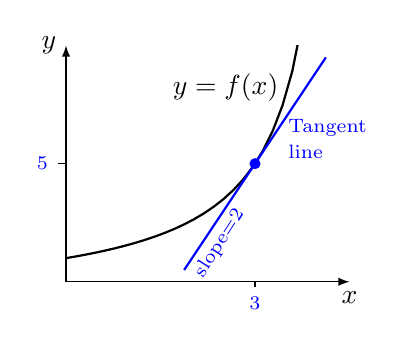
\begin{tikzpicture}[x=12mm,y=6mm,>=latex]
      \draw[black,->] (0,0) -- (3,0) node[below] {$x$};
      \draw[black,->] (0,0) -- (0,5) node[left] {$y$};
      % Ticks:
      \draw[thin,black] (2,0) -- (2,-2pt) node[below,blue] {$\scriptstyle3$};
      \draw[thin,black] (0,2.5) -- (-3pt,2.5) node[left,blue] {$\scriptstyle5$};
      \begin{scope}
        \clip (0,0) rectangle (3,5);
        \draw[black,thick] plot[domain=0:2.5] (\x,{-0.5-3/(\x-3)});
      \end{scope}
      \node[left] at (2.35,{-0.5-3/(2.35-3)}) {$y=f(x)$}; 
      \fill[blue] (2,{-0.5-3/(2-3)}) circle (2pt);
      % Tangent line to y=-0.5-3/(x-3), so y'=3/(x-3)^2 = 3 at x=2.
      % so through (2,2.5) with slope 3; y=3x-3.5
      \draw[thick,blue] (1.25,0.25) -- (2.75,4.75);
      \node[rotate=57.5,blue] at ({1.5+1*0.125},{1-1.5*0.125}) {$\scriptstyle\text{slope}=2$};
      \node[right,blue] at (2.25,3.25) {$\scriptstyle\text{Tangent}$};
      \node[right,blue] at (2.25,2.75) {$\scriptstyle\text{line}$};
    \end{tikzpicture}
  \end{minipage}
  \hfill
  \begin{minipage}{60mm}
    Told $f({\blue 3}) = 5$ and $f{\green '}({\blue 3})={\green 2}$
    \gap

    This means the slope of the tangent line to the graph $y=f(x)$ at $x=3$ is $2$.
    \gap 

    The derivative is this slope, so\ldots
    \gap 

    \fbox{The {\blue units}\ of $\dfrac{dy}{dx}$\ are $\dfrac{\text{units of y}}{\text{units of x}}$}
  \end{minipage}
  \bigskip
  \pause

  \alert{Examples:}

  Heating: derivative units are $\$/{}^{\circ}\ \text{F} = \text{dollars per degree F}$

  Adrenaline: $\text{bpm}/\text{mg} = \text{beats per minute per mg of adrenaline}$.
  \gap

  Units help you understand the {\blue meaning} of the derivative.

}



\frame{
  \frametitle{Interpretation of Derivatives I}

  Suppose $f({\red x})=$ the {\blue percentage of children who still
    get measles} when ${\red x}\%$ of children are inoculated. 
  \gap 

  \alert{Question:}\ Which of the following is a plausible value for $f'(40)$?
  \begin{center}
    A$=0$
    \quad 
    B$= 2$
    \quad 
    C$ = 50$
    \quad 
    D$= -2$
    \quad 
    E$ = -50$
    \pause
    \quad 
    \fbox{D} 
  \end{center}
  \pause
  \gap 

  \alert{Question:}\ If $f({\red 40})={\blue 20}$ and $f'({\red
    40})=-2$, which must be true?
  \begin{itemize}
  \item[A] when 20\% of children are inoculated the  percentage who
    gets measles decreases by $2$\%

  \item[B] when 20\% of children are inoculated then inoculating an
    extra 1\% of children would reduce the number of measles cases by
    another 2\%

  \item[C] If the inoculation rate is 41\% then 18\% of children gets
    measles

  \item[D] If the inoculation rate is 20\% then 2\% fewer cases of
    measles arise if an extra 1\% of children can be inoculated

  \item[E] none of the above
  \pause
  \hfill\alert{Answer:}\ \fbox{C}

  \end{itemize}
}


\frame{
  \frametitle{Interpretation of Derivatives II}

  Air temperature gets colder the higher you go.\\
  $T({\red x})=$ {\blue air temperature} in $^{\circ}C$ at a height $\red x$ meters above sea level.

  \alert{Question:}\ Which of these is a plausible value for $T'({\red 2000})$?
  \begin{center}
    A$ = -1$
    \quad 
    B$ = 1$
    \quad 
    C$ = 0$
    \quad 
    D$ = 1/200$
    \quad 
    E$ = -1/200$
    \pause
    \quad
    \fbox{E} 
  \end{center}
  \pause
  \gap 

  \alert{Question:}\ If $T({\red 2000})={\purple 10}$ and $T{\red'}({\red 2000})=-{\bluegreen 1/200}$, which is most plausible?
  \begin{itemize}
  \item[A] the temperature at sea level is $16^oC$
  \item[B] the temperature $2400$ meters above sea level is $8^oC$
  \item[C] the temperature $10$ meters above sea level is $2000^oC$
  \item[D] 2000 meters above sea level the temperature is decreasing at a rate of $1/200^oC$ per minute.
  \item[E] none of these are plausible
  \end{itemize}
  \pause
  \alert{Answer:}\ \fbox{B}


}



\frame{
  \frametitle{Interpretation of Derivatives III}
  \vspace*{-0.30in}

  \begin{align*}
    {\red x} 
    & = \text{money spent (in thousands of \$) in one month on advertising.}\\
    {\blue f(x)}
    & = \text{{\blue sales} (in thousands of \$) in a month when ${\red x}$ is spent on advertising.}
  \end{align*}
  \pause\vspace*{-0.2in}

  \alert{Question:}\ If $f({\red 20})={\blue 60}$ and $f{\red'}({\red 20})=3$ which must be true?
  \begin{itemize}
  \item[A] When the sales of the company are 20 thousand dollars in
    one month the amount spent on advertising is increasing at a rate
    of 3 thousand dollars per month

  \item[B] When the company spends 20 thousand dollars per month on
    advertising the sales rise at a rate of 3 thousand dollars per
    month 
  \item[C] When the company spends 20 thousand dollars per month on
    advertising each extra dollar a month spent on advertising
    generates an extra 3 dollars of sales. 

  \item[D] When the company spends 3 thousand dollars per month on
    advertising the sales are increasing at a rate of 20 thousand
    dollars per month 

  \item[E] None of the above
    \pause
    \hfill
    \alert{Answer:}\ \fbox{C}
  \end{itemize}

}

\end{document}

\section{Tangent Line Approximations}
\frame{
  \frametitle{\S8.6: Tangent Line Approximation}

  \alert{Question:}\ At 5am the temperature is $42^{\circ}\ \text{F}$ and increasing
  at a rate of $10^{\circ}\ \text{F}$ per hour. Which of the following do you think
  is closest to the temperature at 5:15am? 
  \begin{center}
    A$ = 2.5^{\circ}\ \text{F}$
    \quad 
    B$ = 52^{\circ}\ \text{F}$
    \quad 
    C$ = 43.5^{\circ}\ \text{F}$
    \quad 
    D$ = 44.5^{\circ}\ \text{F}$
    \quad 
    E$ =5.15^{\circ}\ \text{F}$
  \end{center}
  \pause
  \alert{Answer:}\ 
    \fbox{D}

% \gap  5:15 is $1/4$ of an hour after 5am.\\
% $\therefore\quad$ Temperature rises {\blue approximately} $(1/4)\times 10=2.5^{\circ}\ \text{F}$ in this time.\\
% So final temperature is {\blue approximately} $42+2.5=44.5^{\circ}\ \text{F}.$

% \gap
% {\blue Approximately} because instantaneous rate of change is $10$ at $5am$ but this may change. Maybe by 5:10am temperature is increasing at a rate of $11^{\circ}\ \text{F}$ per hour.

% \gap
% Answer is \fbox{{\blue (initial temperature)} + {\red (rise in temperature)}}\\
%  {\red (rise in temperature)} $\approx$ (time taken) $\times$ {\green (rate of change)}
 
%  {\green rate of change} = {\green derivative}

% \gap 
% \includegraphics[scale=0.6]{inputoutput.pdf}

}




\end{document}
